\DiaryEntry{Game of Life - Gardens of Eden}{2022-10-31}{CA}

\subsection{Garden of Eden - Existence}

To analyse Game of Life, we gan look at the game in reverse; instead of investigating what a pattern evolves into, we investigate what evolves into it. That is, we look for parents (and grandparents, and great-grandparents, ...) of the pattern that we are interested in. Some patterns, such as the block, have numerous parents, which is part of the reason why they appear so frequently in the ash of random soups.

Other patterns, such as the clock, have relatively few parents and thus appear less frequently in random soups. Recall that the clock has only six cells and is period 2. Surprisingly, it appears in random soups much less frequently than some much larger objects like the period 3 pulsar or the period 15 pentadecathlon. It seems natural to ask whether or not there exists a pattern that does not have even a single parent. That is, does there exist a pattern that cannot ever appear in the evolution of any other pattern, but rather can only ever appear in generation 0? A pattern with this property is called a \emph{Garden of Eden} and we begin by showing that they do indeed exist.

The rough idea of why Gardens of Eden must exist is that some patterns (such as blocks) have lots of parents, so there are not enough parents left over for all other patterns.

Proof: Let $n \geq 1$ be an integer and consider all patterns that fit within a $6n \times 6n$ square on the Life grid. The contents of the central $(6n - 2) \times (6n - 2)$ square in generation $1$ only depend on the contents of the original $6n \times 6n$ square in generation $0$ (as a cell in generation $n+1$ only depends on neighbours with distance $1$). This central $(6n - 2) \times (6n - 2)$ square contains $(6n - 2)^2$ cells, each of which can be alive or dead, so there are $2^{(6n - 2)^2}$ distinct patterns that could fill this central square. We will now show that, if $n$ is large enough, some of these patterns must have no parent.

To this end, partition the $6n \times 6n$ square into $n^2$ tiles, each of size $6 \times 6$. Each tile contains $36$ cells, each of which can be alive or dead, so there are $2^{36}$ different tiles. However, we can find two tiles which evolve in the same way regardless of what other tiles are placed around them.

The two patterns in generation $0$ look as follows.

\begin{figure}[H]
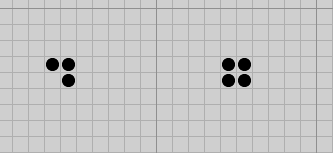
\includegraphics[scale = 0.5]{images/2022-10-31_gol_01.png}
\end{figure}

In generation $1$, the left pattern became the right one.

\begin{figure}[H]
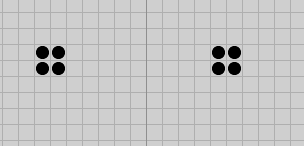
\includegraphics[scale = 0.5]{images/2022-10-31_gol_02.png}
\end{figure}

If we place any pattern with a distance of $2$ around these two $2 \times 2 $ patterns, then the whole pattern will evolve the same (after generation $1$). This is shown in the following two Figures, depicting generation $0$ and generation $1$, respectively.


\begin{figure}[H]
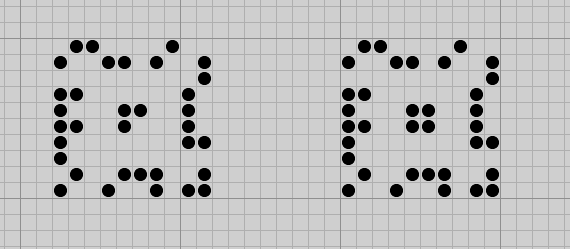
\includegraphics[scale = 0.5]{images/2022-10-31_gol_03.png}
\end{figure}

\begin{figure}[H]
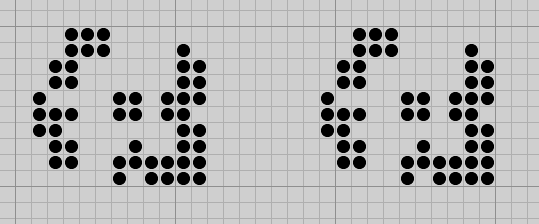
\includegraphics[scale = 0.5]{images/2022-10-31_gol_04.png}
\end{figure}


We thus conclude that in any pattern that uses the first tile, we could replace it by the second tile without changing the evolution of the overall pattern. It follows that if we want to catalog all possible $(6n - 2) \times (6n - 2)$ patterns that can be present in generation $1$, we only need to consider the children of patterns made from a set of $2^{36} - 1$ (and not $2^{36})$ different tiles in generation $0$.

Since the $6n \times 6n$ square has $n^2$ of these tiles, there are at most $(2^{36} - 1)^{n^2}$ different possible  children (i.e., patterns present in generation $1$). Since there are $2^{(6n - 2)^2}$ distinct patterns that could fill the central $(6n - 2) \times (6n - 2)$ square, but at most $(2^{36} - 1)^{n^2}$ of them appear in children of patterns in the $6n \times 6n$ square, all that remains is to show that $(2^{36} - 1)^{n^2} < 2^{(6n - 2)^2}$ when $n$ is sufficiently large. Taking the $n^2$-root of both sides yields $2^{36} - 1 < 2^{(6 - 2/n)^2}$. We can make $2/n$ arbitrarily small and therefore the RHS arbitrarily close to $2^{6^2} = 2^{36}$; in particular, we can make it larger than $2^{36} - 1$ which we wanted to show. \qed

Above proof is very general and did not rely on any particular rules for Game of Life; i.e. it applies to any cellular automata for which two distinct finite patterns evolve into the same pattern.

Now that we know that Gardens of Eden exist, our next goal is to actually find an explicit example of one. Unfortunately, our method of proof is not of much help here, since it only shows that Gardens of Eden exist in extremely large regions (the smallest $n$ for which the inequality $(2^{36} - 1)^{n^2} < 2^{(6n-2)^2}$ holds is somewhere around $n \approx 10^{12}$), and it does not actually tell us how to find one in such a region. The pattern obtained by concatenating together all $2^{n^2}$ different $n \times n$ patterns into a rectangle of size $(n 2^{n^2}) \times n$ is guaranteed to be a Garden of Eden, but it is exponentially larger than the upper bound provided by the theorem.

\subsection{Garden of Eden - Construction}






%%% Local Variables:
%%% mode: latex
%%% TeX-master: "journal"
%%% End:
